\documentclass[11pt, a4paper,titlepage]{article}
\usepackage[utf8]{inputenc}
\usepackage[T1]{fontenc}
\usepackage{fixltx2e}
\usepackage{graphicx}
\usepackage{longtable}
\usepackage{float}
\usepackage{wrapfig}
\usepackage{soul}
\usepackage{textcomp}
\usepackage{marvosym}
\usepackage{wasysym}
\usepackage{latexsym}
\usepackage{hyperref}
\usepackage{amssymb}
\usepackage{hyperref}
\tolerance=1000
\usepackage[left=2.35cm, right=3.35cm, top=3.35cm, bottom=3.35cm]{geometry}
\usepackage[utf8]{inputenc}
\usepackage[greek,english]{babel}
\usepackage{graphicx}
\usepackage{titlesec}
\usepackage{tocbibind}
\providecommand{\alert}[1]{\textbf{#1}}

\begin{document}

\setlength{\parskip}{0pt}%
\setlength{\parindent}{0pt}%
\renewcommand{\thesubsubsection}{\alph{subsubsection}.)}
\begin{titlepage}
  \begin{center}
    
    
\includegraphics[scale=1.5]{Figures/kuleuven_logo.pdf}~\\[4.5cm]
    
    \textsc{\Large Bio-Molecular Model Building}\\[0.5cm]
    
    % Title
    \rule{\linewidth}{0.3mm}\\[0.4cm]
    {\huge \bfseries Exam Exercise} \\[0.4cm]
    {\large Spring 2015} \\[0.4cm]
    \rule{\linewidth}{0.3mm}\\[1.5cm]
    
    % Author and supervisor
    \begin{minipage}{0.4\textwidth}
      \begin{flushleft} \large
        \emph{Author:}\\
        Cedric \textsc{Lood}\\
        Yi Ming \textsc{Gan}\\
      \end{flushleft}
    \end{minipage}
    \begin{minipage}{0.4\textwidth}
      \begin{flushright} \large
        \emph{Supervisors:} \\
        Prof. M. \textsc{De Maeyer}\\
        dr. J. \textsc{De Raeymaecker}\\
        dr. X. \textsc{Qing}
      \end{flushright}
    \end{minipage}
    
    \vfill
    
    
\includegraphics[scale=0.15]{Figures/KUL.jpg}~\\[0.5cm]

    % Bottom of the page
    {\large \today}
    
  \end{center}
\end{titlepage}

\setcounter{tocdepth}{3}
\tableofcontents
\clearpage


\section{Question 1 - Kinases}
\subsection{Part a}
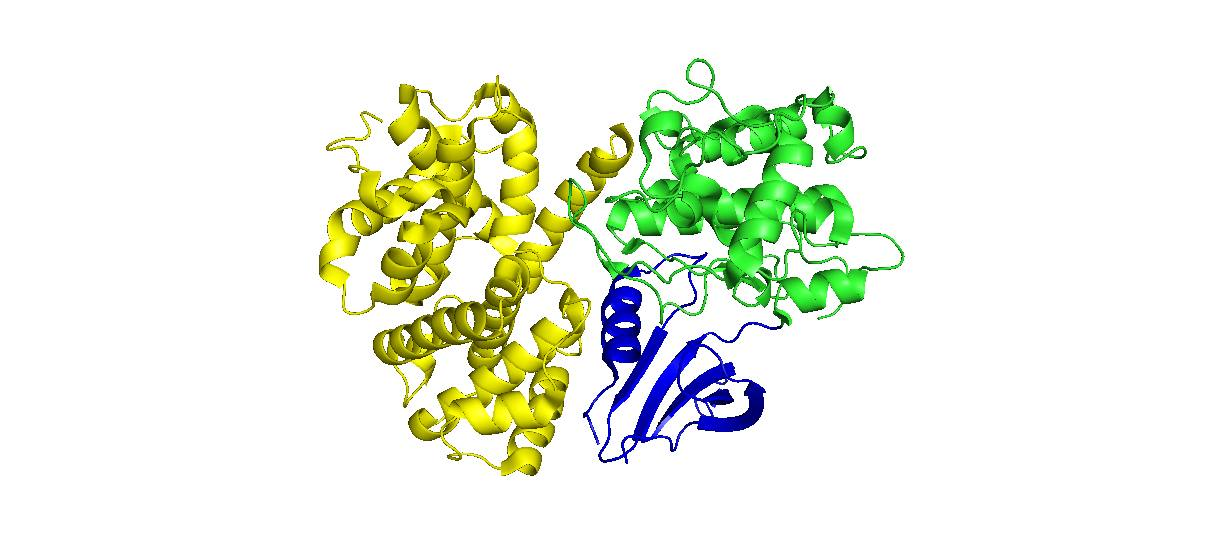
\includegraphics[width=15cm]{./Figures/1a.jpg}

\subsection{Part b}
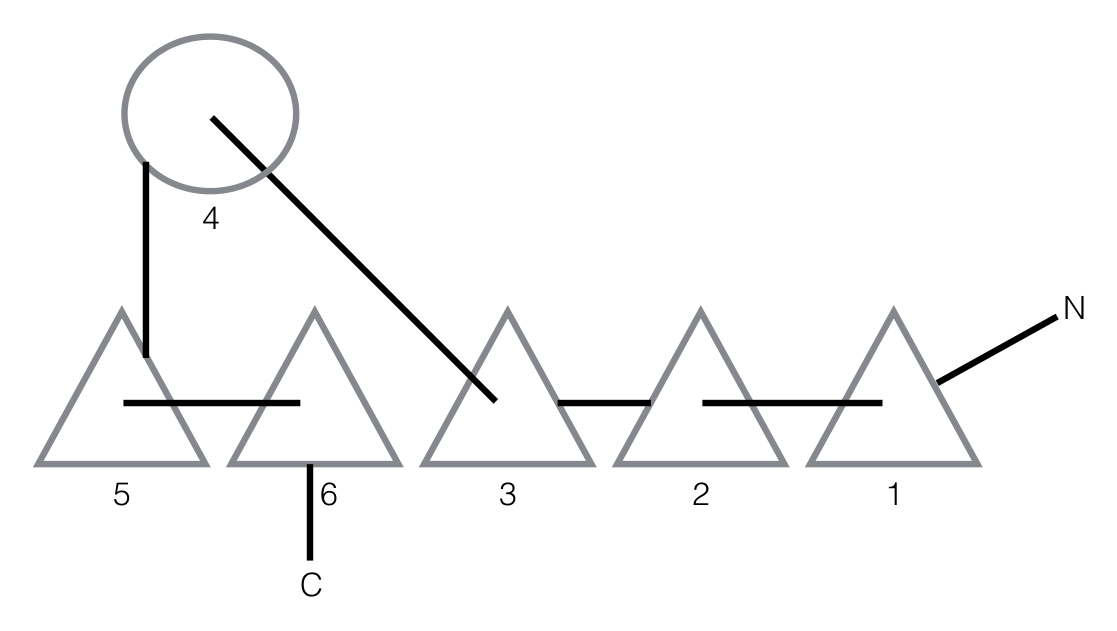
\includegraphics[width=12cm]{./Figures/1b.png}

\section{Question 2 - Kinase active/inactive forms}
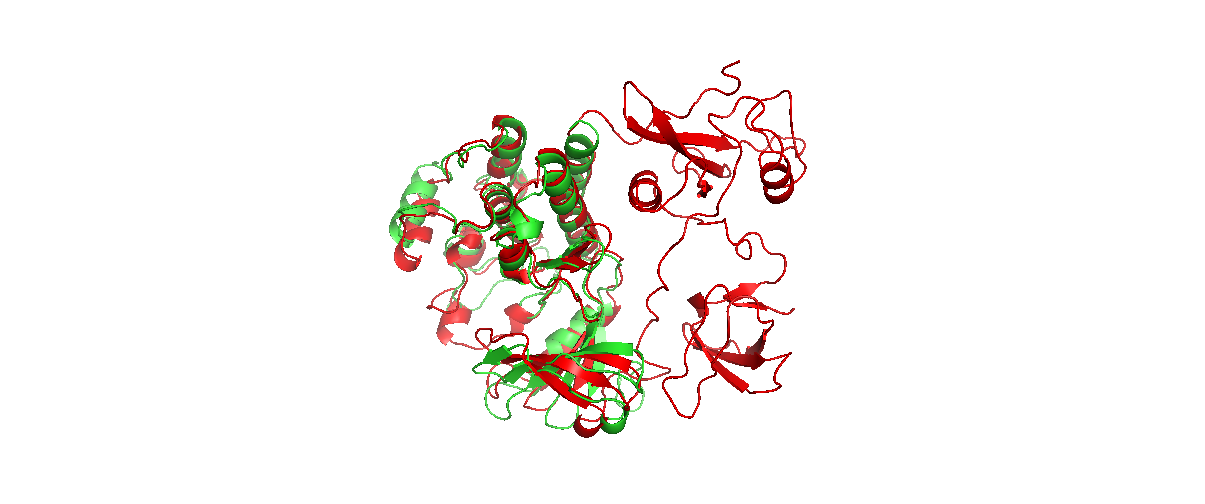
\includegraphics[width=15cm]{./Figures/2a.png}

The role of regulatory domains in the kinases are to induce
conformational changes that switch the kinase from one form (inactive
or active) to the other \cite{ConformationalPlasticityKinases}.

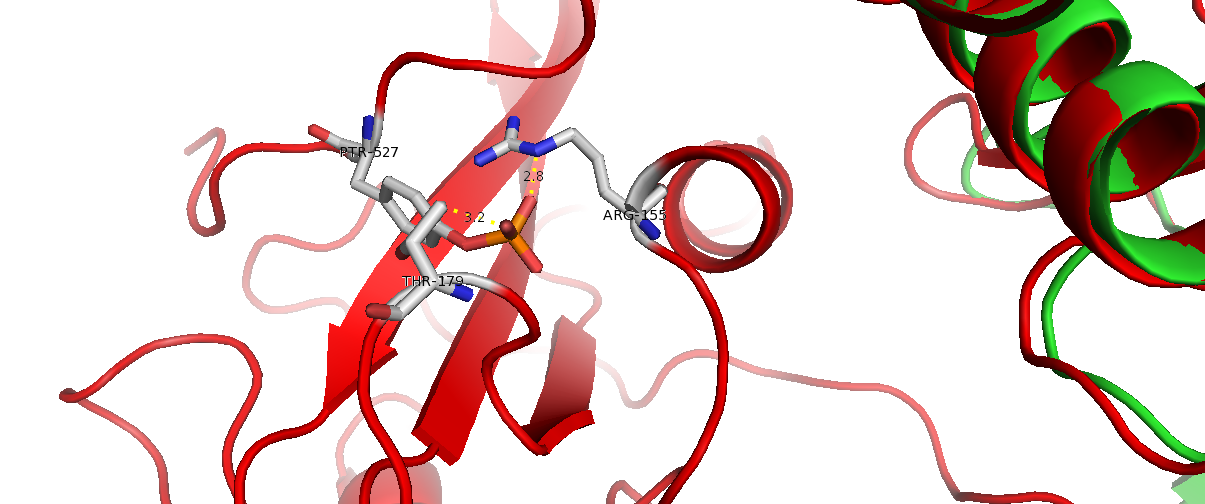
\includegraphics[width=15cm]{./Figures/2b.png}

\section{Question 3}

\begin{verbatim}
> table(years)
years
2000 2001 2002 2003 2004 2005 2006 2007 2008 2009 2010 2011 2012 2013 2014 2015 
  41   84   91  131  123  192  224  298  329  309  348  316  426  402  358  102 
> barplot(table(years))
\end{verbatim}

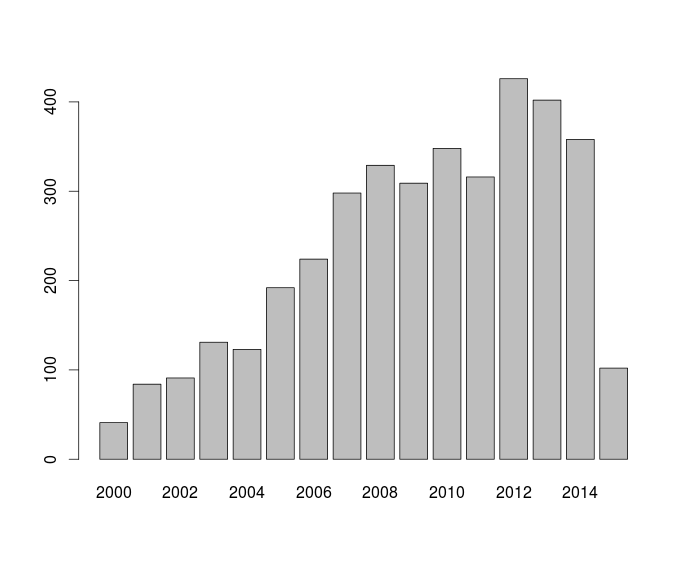
\includegraphics[width=12cm]{./Figures/pdb_kinases_growth.png}

\section{Question 4}
\subsection{Part a}

The molecule bound is Phosphoaminophosphonic Acid-Adenylate Ester, or
ANP. Along with 2 Magnesium Ions.

\subsection{Part b}
ANP is an analog of ATP that cannot be hydrolized by the
kinase. Therefore it stays bound to the active site of the kinase and
allows for the crystal structure of the molecule to be established.

\subsection{Part c}

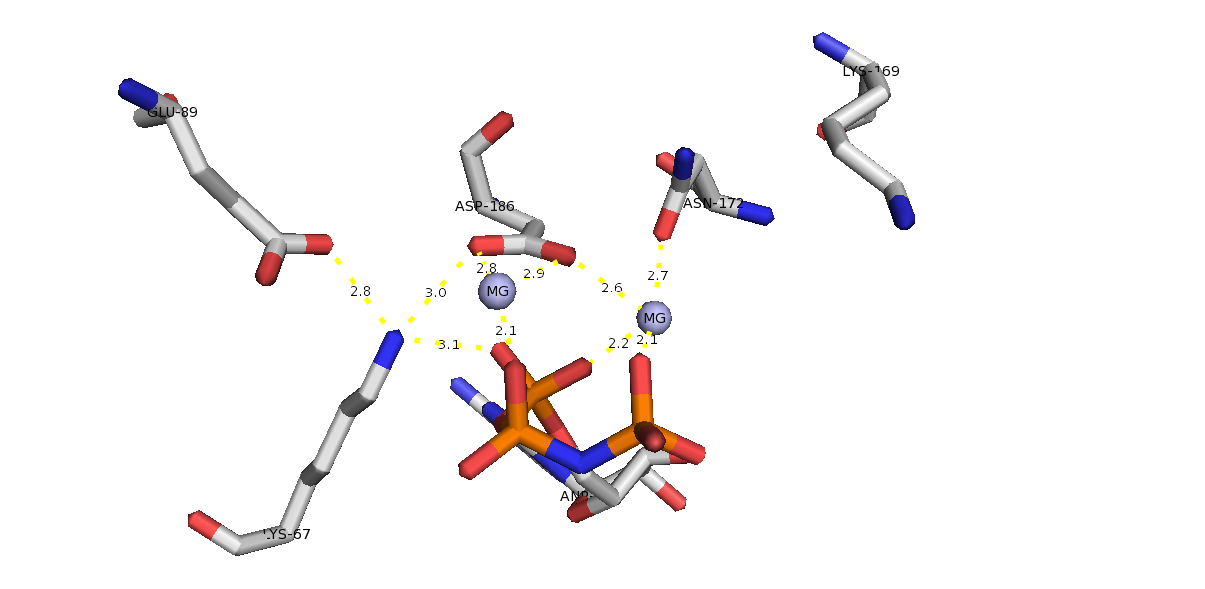
\includegraphics[width=15cm]{./Figures/4c.png}

As shown in the figure, a salt bridge is formed between Glu89 and
Lys67.  Lys67 forms a salt bridge directly with the $\alpha$-phosphate
oxygen of the ANP molecule. Asp186 forms H-Bond with the Lys67 and
also coordinates the Magnesium Ion, that in turns coordinates the
$\beta$-phosphate oxygen of the ANP molecule. Asn172, in collaboration
with Asp186 coordinates the second Magnesium Ion which interacts with
the $\alpha$ and $\gamma$-phosphate oxygens of the ANP molecule
\cite{CSPim1Kinase}.

\subsection{Part d}

The AUTHOR section from the PDB file reveals the same list of names as
the list of the article's authors:

\begin{verbatim}
AUTHOR    K.C.QIAN,L.WANG,E.R.HICKEY,J.STUDTS,K.BARRINGER,C.PENG,               
AUTHOR   2 A.KRONKAITIS,J.LI,A.WHITE,S.MISCHE,B.FARMER         
\end{verbatim}
 
\section{Question 5}
We found 2 proteins of interest: 1JKK and 3F5U. Both have reasonable
resolutions and R-Free values are similar. 1JKK boasts a 'up to 1.5 A'
resolution of the catalytic domain. However, after visualizing the
B-Factors using pymol, we decided to go with 3F5U.

\subsection{Part a}
The AUTHOR section from the PDB file reveals the same list of names as
the list of the article's authors:

\begin{verbatim}
AUTHOR    L.K.MCNAMARA,D.M.WATTERSON,J.S.BRUNZELLE
\end{verbatim}

\subsection{Part b}
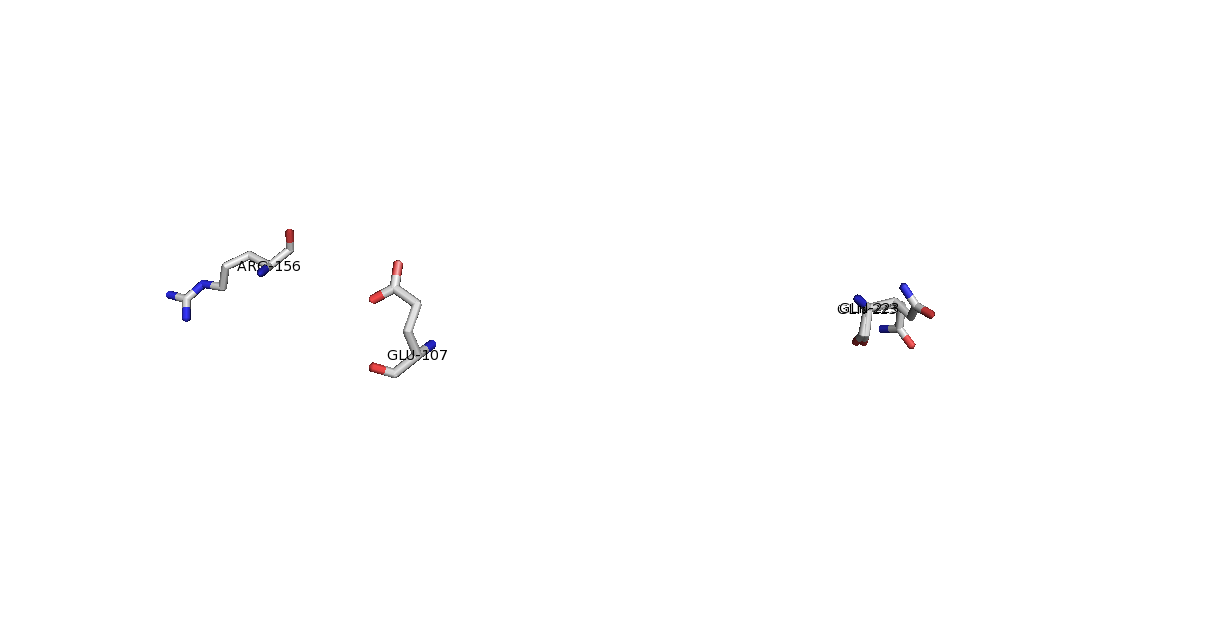
\includegraphics[width=15cm]{./Figures/5b.png}

\subsection{Part c}

Overall, this structure has low B-factors. There is however a loop
region, located around amino acids 291-294, which displays higher
B-Factors (around 100). The reason for this seems to be lying in the
fact that this loop is part of a flexible regions at the C-Terminus,
which is not captured by the X-Ray crystalography.

\subsection{Part b}
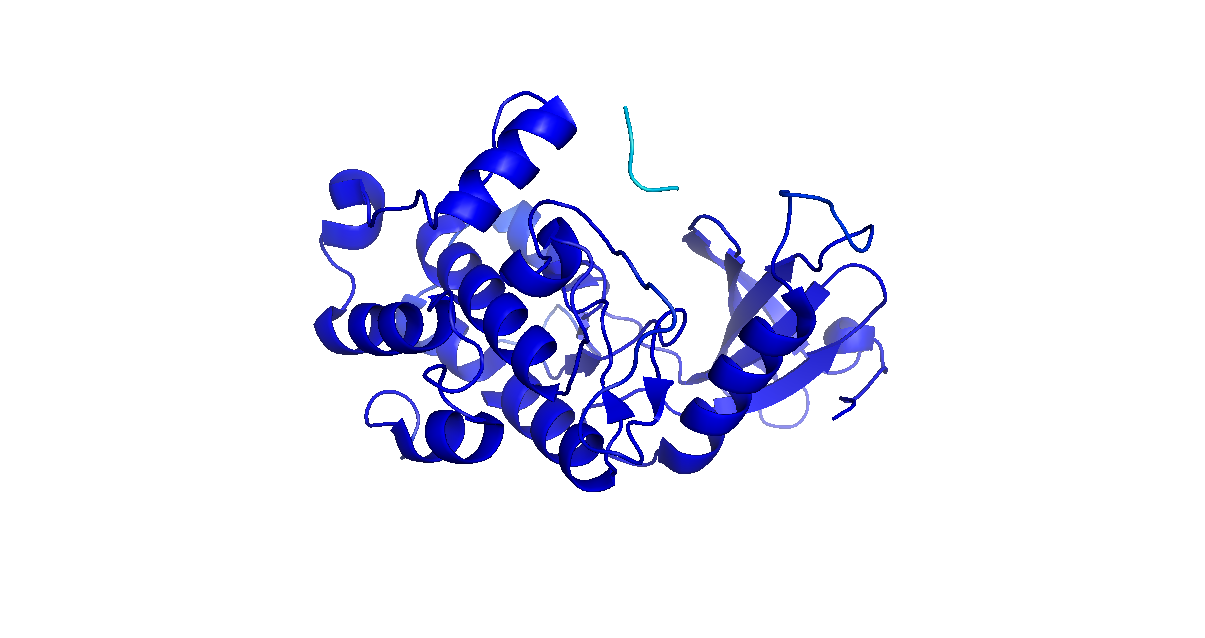
\includegraphics[width=15cm]{./Figures/5c.png}

\subsection{Part d}
The domains present in DPAK1-Human
\url{http://www.uniprot.org/uniprot/P53355} are:

\begin{itemize}
\item Kinase whose function is to catalize the transfer of phosphate
  groups to specific substrates.
\item Ankyrin domains (multiple found) mediate protein-protein
  interactions.
  \url{https://en.wikipedia.org/wiki/Ankyrin_repeat}
\item Roc domain, which is a GTPase domain. GTP binding to the ROC
  domain activates kinase activity.
  \url{http://www.copewithcytokines.de/cope.cgi?key=ROC%20domain} 
\item The death domain (DD) is a protein interaction module composed
  of a bundle of six alpha-helices.
  \url{https://en.wikipedia.org/wiki/Death_domain}
\end{itemize}
\subsection{Part e}
\bibliographystyle{plain}
\bibliography{bib-db}
\end{document}
